\section{Adaptive Telemetry and Radio Power Model}

To preserve aircraft battery endurance while maintaining operational situation awareness, MANAR defines an adaptive telemetry transmission model. This section formalizes the radio power consumption model as a function of stream frequency and establishes a multi-tiered transmission rate policy.

\subsection{Analytical Radio Telemetry Power Model}
Radio frequency (RF) telemetry power consumption scales with transmission duty cycle. Let $P_{\mathrm{TX}}$ denote transmitter active power, $P_{\mathrm{RX}}$ denote receiver baseline power, and $R$ denote link channel data rate in bits per second (bps). 

For a telemetry stream $i$ with message payload size $B_i$ (bytes) transmitted at frequency $f_i$ (Hz), the incremental electrical radio power $\Delta P_i$ consumed over the idle/receive baseline is formulated as:
\begin{equation}
\Delta P_i = (P_{\mathrm{TX}} - P_{\mathrm{RX}}) \cdot \left(\frac{8 \cdot B_i \cdot f_i}{R}\right) = \beta \cdot B_i \cdot f_i
\end{equation}
where $\beta$ is the radio transmission slope coefficient:
\begin{equation}
\beta = \frac{(P_{\mathrm{TX}} - P_{\mathrm{RX}}) \cdot 8}{R} \quad \left(\frac{\text{W}}{\text{byte} \cdot \text{Hz}}\right)
\end{equation}

For a reference UHF/cellular telemetry link with $P_{\mathrm{TX}} = 4.80\text{ W}$, $P_{\mathrm{RX}} = 0.36\text{ W}$, and channel rate $R = 64\,000\text{ bit/s}$, the slope coefficient evaluates to $\beta \approx 5.55 \times 10^{-4}\text{ W}/(\text{byte}\cdot\text{Hz})$.

Fig.~\ref{fig:manar_telemetry_power_frequency} illustrates the incremental radio power across transmission frequencies from $0$ to $10\text{ Hz}$ for fourteen distinct MANAR telemetry message categories.

\begin{figure}[t]
\centering
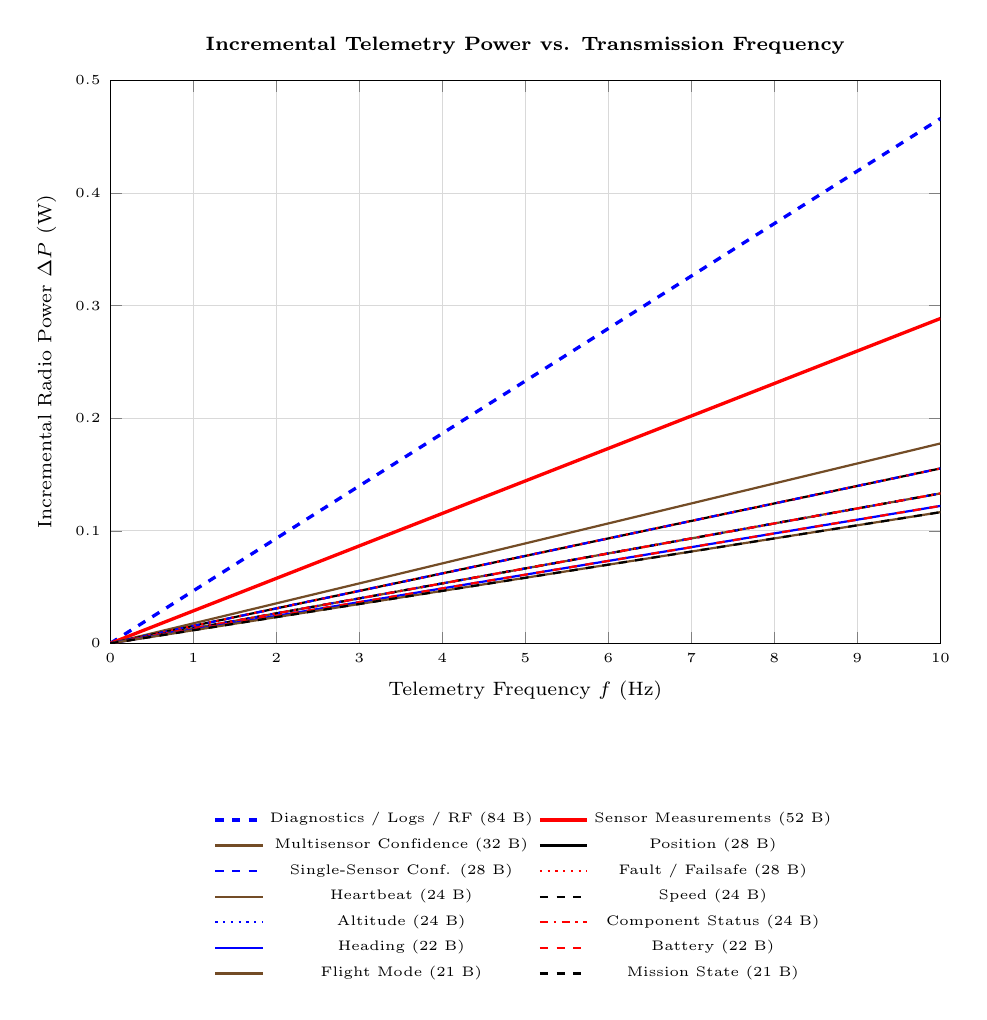
\begin{tikzpicture}
    \begin{axis}[
        width=\columnwidth,
        height=0.72\columnwidth,
        xlabel={Telemetry Frequency $f$ (Hz)},
        ylabel={Incremental Radio Power $\Delta P$ (W)},
        xmin=0,
        xmax=10,
        ymin=0,
        ymax=0.50,
        grid=both,
        minor grid style={gray!15},
        major grid style={gray!30},
        tick label style={font=\tiny},
        label style={font=\scriptsize},
        title style={font=\scriptsize\bfseries},
        legend style={
            font=\tiny,
            at={(0.5,-0.28)},
            anchor=north,
            legend columns=2,
            draw=none
        },
        title={Incremental Telemetry Power vs. Transmission Frequency}
    ]

    % Diagnostics / logs / RF history / config: 84 bytes
    \addplot+[very thick, dashed, no markers, domain=0:10]
        {0.04662*x};
    \addlegendentry{Diagnostics / Logs / RF (84 B)}

    % Sensor measurements: 52 bytes
    \addplot+[very thick, solid, no markers, domain=0:10]
        {0.02886*x};
    \addlegendentry{Sensor Measurements (52 B)}

    % Multisensor confidence event: 32 bytes
    \addplot+[thick, solid, no markers, domain=0:10]
        {0.01776*x};
    \addlegendentry{Multisensor Confidence (32 B)}

    % Position: 28 bytes
    \addplot+[thick, solid, no markers, domain=0:10]
        {0.01554*x};
    \addlegendentry{Position (28 B)}

    % Single-sensor confidence event: 28 bytes
    \addplot+[thick, dashed, no markers, domain=0:10]
        {0.01554*x};
    \addlegendentry{Single-Sensor Conf. (28 B)}

    % Fault / failsafe: 28 bytes
    \addplot+[thick, dotted, no markers, domain=0:10]
        {0.01554*x};
    \addlegendentry{Fault / Failsafe (28 B)}

    % Heartbeat: 24 bytes
    \addplot+[thick, solid, no markers, domain=0:10]
        {0.01332*x};
    \addlegendentry{Heartbeat (24 B)}

    % Speed: 24 bytes
    \addplot+[thick, dashed, no markers, domain=0:10]
        {0.01332*x};
    \addlegendentry{Speed (24 B)}

    % Altitude: 24 bytes
    \addplot+[thick, dotted, no markers, domain=0:10]
        {0.01332*x};
    \addlegendentry{Altitude (24 B)}

    % Component status: 24 bytes
    \addplot+[thick, dashdotted, no markers, domain=0:10]
        {0.01332*x};
    \addlegendentry{Component Status (24 B)}

    % Heading: 22 bytes
    \addplot+[thick, solid, no markers, domain=0:10]
        {0.01221*x};
    \addlegendentry{Heading (22 B)}

    % Battery: 22 bytes
    \addplot+[thick, dashed, no markers, domain=0:10]
        {0.01221*x};
    \addlegendentry{Battery (22 B)}

    % Flight mode: 21 bytes
    \addplot+[thick, solid, no markers, domain=0:10]
        {0.011655*x};
    \addlegendentry{Flight Mode (21 B)}

    % Mission state: 21 bytes
    \addplot+[thick, dashed, no markers, domain=0:10]
        {0.011655*x};
    \addlegendentry{Mission State (21 B)}

    \end{axis}
\end{tikzpicture}
\caption{Analytical estimate of incremental radio power for individual MANAR telemetry message types across transmission frequencies ($P_{\mathrm{TX}} = 4.8\text{ W}$, $P_{\mathrm{RX}} = 0.36\text{ W}$, $R = 64\text{ kbps}$).}
\label{fig:manar_telemetry_power_frequency}
\end{figure}

\subsection{Adaptive Transmission Rate Policy}
To minimize RF power overhead during transit while providing high-bandwidth telemetry during active victim localization, MANAR implements a dual-regime rate policy. Table~\ref{tab:telemetry_rates} defines the transmission rates for all telemetry streams under normal search vs. proximity/critical operations.

\begin{table*}[t]
\caption{MANAR Adaptive Telemetry Rate Policy and Operational Rationale}
\label{tab:telemetry_rates}
\centering
\footnotesize
\begin{tabularx}{\textwidth}{@{}clcccX@{}}
\toprule
\textbf{Tier} & \textbf{Telemetry Stream} & \textbf{Payload ($B_i$)} & \textbf{Normal Rate} & \textbf{Proximity / Critical Rate} & \textbf{Operational Rationale} \\
\midrule
\textcolor{green!60!black}{\ding{108}} & \textbf{Heartbeat} & 24 B & 2.0 Hz & 2.0 Hz & Low-overhead link-health and watchdog awareness. \\
\textcolor{green!60!black}{\ding{108}} & \textbf{Position} & 28 B & 2.0 Hz & 5.0 Hz & Primary navigation telemetry; modest radio power cost. \\
\textcolor{green!60!black}{\ding{108}} & \textbf{Speed} & 24 B & 2.0 Hz & 5.0 Hz & Low power footprint; useful for live kinematic context. \\
\textcolor{green!60!black}{\ding{108}} & \textbf{Altitude} & 24 B & 2.0 Hz & 5.0 Hz & Critical for terrain clearance and vertical safety. \\
\textcolor{green!60!black}{\ding{108}} & \textbf{Heading} & 22 B & 1.0 Hz & 5.0 Hz & Low marginal cost; 1 Hz baseline sufficient in transit. \\
\midrule
\textcolor{blue!80!black}{\ding{108}} & \textbf{Battery Percentage} & 22 B & 0.2 Hz & 0.5 Hz & 5-second interval sufficient under normal discharge. \\
\midrule
\textcolor{yellow!70!black}{\ding{108}} & \textbf{Flight Mode} & 21 B & On change & On change & Event-driven update; redundant transmissions avoided. \\
\textcolor{yellow!70!black}{\ding{108}} & \textbf{Mission State} & 21 B & On change & On change & State transition telemetry published on event trigger. \\
\textcolor{yellow!70!black}{\ding{108}} & \textbf{Component Status} & 24 B & On change / fault & Active components only & Payload status updates sent on state modification. \\
\midrule
\textcolor{orange!90!black}{\ding{108}} & \textbf{Sensor Measurements} & 52 B & Local only & 5.0--10.0 Hz & High-rate raw sensor data streamed only in proximity. \\
\textcolor{orange!90!black}{\ding{108}} & \textbf{Single-Sensor Confidence} & 28 B & Immediate event & Stream relevant sensor & Triggered immediately upon validated detection event. \\
\midrule
\textcolor{red!80!black}{\ding{108}} & \textbf{Multisensor Confidence} & 32 B & Immediate event & Trigger proximity mode & High-priority event; escalates system telemetry tier. \\
\textcolor{red!80!black}{\ding{108}} & \textbf{Fault / Failsafe / Low Batt} & 28 B & Immediate event & Repeat while active & Emergency telemetry; bypasses normal bandwidth caps. \\
\midrule
\textcolor{gray!80!black}{\ding{108}} & \textbf{Diagnostics / Logs / Config} & 84 B & On-demand & On-demand & High payload footprint; retrieved only on operator query. \\
\bottomrule
\end{tabularx}
\end{table*}

Under normal cruise and transit search phases, routine navigation streams (position, speed, altitude) update at $2\text{ Hz}$, while slow-varying state like battery percentage is throttled to $0.2\text{ Hz}$ ($5\text{ s}$ intervals), and discrete states transmit strictly upon change. When candidate evidence triggers a single-sensor or multisensor confidence event, the system dynamically escalates to the proximity rate regime ($5\text{--}10\text{ Hz}$), allocating RF bandwidth and power specifically when localization fidelity is paramount.
